\documentclass{whutmod}
\usepackage{metalogo}
\usepackage{float}
\usepackage{subfigure} 
\usepackage{url}
\usepackage{booktabs}
\bibliographystyle{unsrt}
\team{23}
\membera{刘子川}
\joba{编程}
\memberb{程宇}
\jobb{建模}
\memberc{陈荣兴}
\jobc{建模}
\hypersetup{
	colorlinks=true,
	linkcolor=black
}

\title{基于因子分析与灰色关联分析对武汉市人才吸引力的量化评价}
\tihao{4} 

\begin{document}

	%\maketitle
	
	\begin{abstract}

植物的种类繁多,为研究植物分类方法,本文基于植物树叶的二值化图片数据,通过\textbf{解析几何计算}和\textbf{时间序列展开}的方法转换成轮廓特征向量和边缘特征向量;再通过\textbf{粒子群算法}优化的\textbf{深度神经网络}解决树叶识别分类问题,并分析核心指标对模型性能的影响,最终结合树叶纹理信息对模型进行改进和分析比较。
~\\

针对问题一,通过\textbf{解析几何计算}和\textbf{时间序列展开},分别提取每一张图片中的特征向量。根据题目要求,本组首先利用\textbf{matlab}计算与图像形状相关的解析几何特征量,得到由八个几何学、拓扑学特征值组成的\textbf{八维}形状特征向量。然后将图像轮廓进行极化投影,并通过\textbf{numpy工具箱}将极化投影轮廓展开成时间序列,挖掘分析时间序列的三个特征值,组成\textbf{三维}边缘特征向量。最后合并两个向量得到\textbf{十一维}总体特征向量。~\\


针对问题二,基于问题一中提取的特征信息,建立了\textbf{PSO-DNN网络}对树叶进行识别与分类。利用\textbf{Keras工具库}搭建\textbf{深度神经网络},利用\textbf{粒子群算法}优化DNN网络的连接权值和阈值,对研究对象进行识别分类。训练后的神经网络模型预测准确率为$\textbf{91.037\%}$,并分析各指标的权重占比,判断出特征量中\textbf{时间序列熵、密实度和最大压痕深度}对模型性能影响最大,是模型的核心指标。将其剔除后,模型分类精确度损失率分别为\textbf{6.937\%、5.498\%、3.559\%}。
~\\

针对问题三,基于问题二中的\textbf{PSO-DNN网络}模型,将树叶纹理信息嵌入特征向量。增加网络输入层个数,并对模型进行参数调整,最终得到叶片的预测准确率达到$\textbf{96.634\%}$。
~\\

本文中所提到的模型优点主要有两点:一、提取的特征值信息包含量大、区分度高;二、利用PSO优化后的DNN网络全局收敛能力强,分类准确度高。

	
  
\keywords{时间序列展开\quad  深度神经网络\quad  粒子群算法\quad Keras工具库\quad }
		
	\end{abstract}
	
	%目录
	\tableofcontents
	\newpage	%换页符
	
	\section{问题重述}	
	\subsection{问题背景}
    诺曼底登陆:代号“霸王行动”,是第二次世界大战中盟军在欧洲西线战场发起的一场大规模攻势,接近三百万士兵渡过英吉利海峡前往法国诺曼底。诺曼底战役是人类战争史上规模最大的一次海上登陆战役行动,使第二次世界大战的战略态势发生了根本性的变化。
    
    海运装载是海上登陆战役中的一种作战行动,将需要登陆的部队人员、装备、补给品装载到海上运输工具,该行动会直接影响着登陆作战效果。以诺曼底战役的第一批海上登陆输送兵力为参考,不同成建制单位的部队人员、装备和补给品都有不同的数量级需求,研究合理利用海军运输船和民用船只进行兵力装载以及对装载方案的优化都具有重要意义。
    
    
    

	\subsection{问题概述}
    围绕相关附件和条件要求,研究海运装载行动输送兵力任务的合理安排,依次提出以下问题:
		 
	
	\textbf{问题一:}根据输送任务和海上运输工具情况,结合相关条件和要求,分析运输船舰和兵力的关系,概算各类型旅一个旅级单位的运输工具的需求量,并给出具体装载方案。
	
	\textbf{问题二:}根据输送任务,结合附件中的港口及码头泊位,制定时间最短、船只数量最少的兵力装载方案。
	
	\textbf{问题三:}假设装载行动开始24小时后,A港口的两个A1和一个A2泊位,D港口的一个D2和两个D3泊位被毁,给出具体调整方案以及完成装载任务的对策建议。
	
	
	\section{模型假设}
	\begin{itemize}                                             
		\item [(1)] 为了简化计算,假设题目中给出的模糊数据都是精确数据。
		\item [(2)] 为了优化运算结果,假设所有全副武装的士兵都保持坐姿休息。
		\item [(3)] 假设在战争中,装载消耗更少时间的优先度高于使用更少的民用船。
		\item [(4)] 假设在装载过程中,同一泊口的船舰装载交替时间可以忽略不记。
		\item [(5)] 假设港口被摧毁时,由于提前得到信息,港口上的船只与兵力没有损失,只是正在进行的装载工作停止,且进度完全损失。
	\end{itemize}
	
	
	\section{符号说明}
%	每行都有线的表
%	\begin{center}
%		\begin{tabular}{cc}
%			\hline
%			\makebox[0.3\textwidth][c]{符号}	&  \makebox[0.4\textwidth][c]{意义} \\ \hline
%			$C_{0}$	    &  污染源初始浓度 \\ \hline
%			$C(x,t)$	    &  污染浓度随时空变化 \\ \hline
%			$u_{x}$	    &  江河平均纵向流速 \\ \hline
%			$E_{x}$  &  铊在江河纵向弥散系数\\ \hline
%		$p$   &  面污染物纵向距离\\ \hline
%			$K_{c}$	    & 污染物降解系数  \\ \hline
%		    $a$	& 污染超标系数 \\ \hline
%		     $x$	& 距污染源的一维距离 \\ \hline
%		      $t$	& 距污染发生后的时间 \\ \hline
%		       $V_{A}$	& 溶液摩尔体积 \\ \hline
%		      $M_{B}$	& 江水的摩尔质量 \\ \hline
%		     $\mu_{B}$	& 溶剂的粘度 \\ \hline		      
%		\end{tabular}
%	\end{center}

%三线表
	\begin{table}[H]
	\label{biao} \centering
		\begin{tabular}{cc}
			\toprule[1.5pt]
			\multicolumn{1}{m{5cm}}{\centering 符号} & \multicolumn{1}{m{5cm}}{\centering 说明} \\
			\midrule[1pt]
			$I$  &  研究图像 \\ 
			$A(I)$  &  图像面积 \\ 
			$C(I)$  & 图像几何中心\\
			$\partial I$  &  图像边界 \\ 
		    $d(.)$ & 运算两点间欧式距离\\
			$ID$	 &  总特征向量  \\ 
			$ID_{shape}$ &  形状特征向量 \\ 
			$ID_{margin}$	 &  边缘特征向量 \\ 
			$id_{k}$  &   研究图像特征值\\ 
			$r$  &  极径\\	
			$\theta$ & 极角\\
			$X$ &  时间序列集\\ 
			$S$ & shapelet子序列\\
			$x_{i}$ & 神经网络第$i$个输入值\\
			$w_{ki}$ & 第$i$个输入量连接的权值\\
			$b_{k}$ & 神经网络阈值\\
			$f$  & 激活函数\\
			$e$ & 误差函数\\
			$E$ & 全局误差\\
			$\eta $ &  学习率\\
			$c_{1,2}$ & 加速因子\\
			$\beta$ & 惯性权重\\
			

		
			\bottomrule[1.5pt]
		\end{tabular}
	\end{table}

	\section{问题一模型的建立与求解}

    \subsection{问题描述与分析}

    问题一要求根据输送任务和船舰情况,结合相关条件和要求,分析运输船舰和兵力的关系,概算各类型旅一个旅级单位对船舰的需求量,给出装载方案。其本质是一个多背包优化问题,要求使用尽可能少的背包,装载各种旅的一个旅编制兵力。本组首先对兵力、装备与装载的面积进行量化,根据题目要求,以派出船舰种类和数量作为决策向量,以所用的总船只数量为目标函数,设计沙石算法,使得每艘船面积利用率达到最高,从而调用船支数达到最小值。
    

	    \subsection{模型的建立}
	    \subsubsection{兵力、装备与船载的面积量化}


	    计算附件2中的每种装备与所占面积,得到装备占用面积向量:
	    \begin{gather*}
	    s_{xi}=l_{i}\times w_{i} \times \varepsilon _{i}\\
	        S_{x}=[s_{x1},s_{x2},\cdots,s_{x14}]
	    \end{gather*}
	    其中$s_{xi}$是装备$X_{i}(i=1,2\cdots,14)$的占用面积,$l_{i}$、$w_{i}$与$\varepsilon _{i}$分别是装备$X_{i}$的长、宽与面积修正系数。
	    
	     计算附件2中每种旅一个营的占用面积,得到每营人口所占面积向量:


	     \begin{gather*}
	     s_{pi}=p_{i}\times s\\
	     S_{p}=[s_{p1},s_{p2},\cdots,s_{p12}]
	     \end{gather*}
	     其中$p_{i}$是第$i(i=1,2,\cdots,12)$的全副武装人员数,取$s=0.5m^2$为每个全副武装人员占用的面积。
	     
	     计算附件3中登陆舰可用装载面积,得到登陆舰有效面积向量:
	      \begin{gather*}
	      s_{yi}=s_{i}\times \eta_{1}\\
	      S_{y}=[s_{y1},s_{y2},\cdots,s_{y14}]
	      \end{gather*}
	    其中$s_{yi}$是登陆舰$Y_{i}(i=1,2\cdots,14)$的可用装载面积,$s_{i}$是登陆舰$Y_{i}$的总装载面积,取$\eta_{1}=75\%$为登陆舰的有效面积率。
	    
	    计算附件3中民用船可用装载面积,得到登陆舰有效面积向量:
	      \begin{gather*}
	      s_{zj}=s_{j}\times \eta_{2}\\
	      S_{z}=[s_{z1},s_{z2},\cdots,s_{z5}]
	      \end{gather*}
	       其中$s_{zi}$民用船$Z_{j}(i=1,2\cdots,5)$的可用装载面积,$s_{j}$是民用船$Z_{j}$的总装载面积,取$\eta_{2}=70\%$为民用船只的有效面积率。
	    \subsubsection{优化函数与约束条件}
	    令$y_{k} $ $(k=1,2,\cdots ,14)$为派出的登陆舰数量,$z_{n}$$(n=1,2,\cdots ,5)$为派出民用船的数量,建立\textbf{决策向量}:
	     \begin{gather*}
	     D=[y_{1},y_{2},\cdots,y_{14},z_{1},z_{2},\cdots,z_{5}]
	    \end{gather*}
	    
	    
	    根据题意尽可能使用少的船舰数,即\textbf{目标函数}为使用船舰总数:
	     \begin{gather}
	    min Z=\sum _{1}^{19}D[k]
	  \end{gather}
	    
	    
	   其中舰载面积系数向量为:
	    \begin{gather*}
	    S_{D}=[S_{y}, S_{z}]
    	\end{gather*}
    	
    	根据题目要求总舰载有效面积不小于总兵力装备占用面积:
    	 \begin{gather*}
    	 D\cdot S_{D}\geq \sum  S_{x} + \sum  S_{p}
    	 \end{gather*}
    	 
    	 且由登陆舰Y1的有效舰载面积大于装备X9(直升机)的部队占用的面积,其中$\sum  s_{p6}$是唯一装备的部队—$\uppercase\expandafter{\romannumeral6}$旅的人口总和:
    	  \begin{gather*}
    	 y_{1}\cdot s_{y1}\geq \sum s_{x9}+ \sum  s_{p6}
    	 \end{gather*}
    	 
    	 

    	 综上,建立得到使用最少船舰装载每种旅各一个旅级编制的\textbf{模型}为:
    	  \begin{gather}
    	 min Z=\sum _{1}^{19}D[k]\\ 
    	  s.t.\left\{\begin{matrix}	 D\cdot S_{D}\geq \sum  S_{x} + \sum  S_{p}
    	 \\ y_{1}\cdot s_{y1}\geq \sum s_{x9}+ \sum  s_{p6}
    	 \\S_{D}=[S_{y}, S_{z}]
    	 \\ s_{xi}=l_{i}\times w_{i} \times \varepsilon _{i}
    	 \\S_{x}=[s_{x1},s_{x2},\cdots,s_{x14}]
    	 \\s_{pi}=p_{i}\times s
    	 \\S_{p}=[s_{p1},s_{p2},\cdots,s_{p12}]
    	 \\     s_{yi}=s_{i}\times \eta_{1}
    	 \\   S_{y}=[s_{y1},s_{y2},\cdots,s_{y14}]
    	 \\      s_{zj}=s_{j}\times \eta_{2}
    	 \\ S_{z}=[s_{z1},s_{z2},\cdots,s_{z5}]
    	 \end{matrix}\right. 
     	 \end{gather}

    		    	
	\subsection{模型的求解}   
    	  \subsubsection{沙石算法}

		为使得调用的船舰数量最少,即需使得每艘船的未利用面积值达到最小:
	    \begin{gather}
		min \Delta S= \sum  S_{x} + \sum  S_{p}-D\cdot S_{D} 
		\end{gather}
	其中$\Delta S$为损失面积,本组设计沙石算法优化部队装载方案,使其得面积损失达到最小,具体如下:
	 \paragraph{算法思想}
	 根据经验,使用沙砾和石子填满某个刚性容器,较好的方法是先装入石子,后灌入沙砾,可以让剩余空间达到最小。基于此,本组设计\textbf{沙石算法},将带待装载部队(其占用面积不尽相同)视作沙砾与石子,将船舰视作刚性容器,即可求出面积利用率最高的部队装载方案。沙石算法示意图如图 ~\ref{shashi}~所示:
	 
	 
	 \begin{figure}[H]
	 	\centering
	 	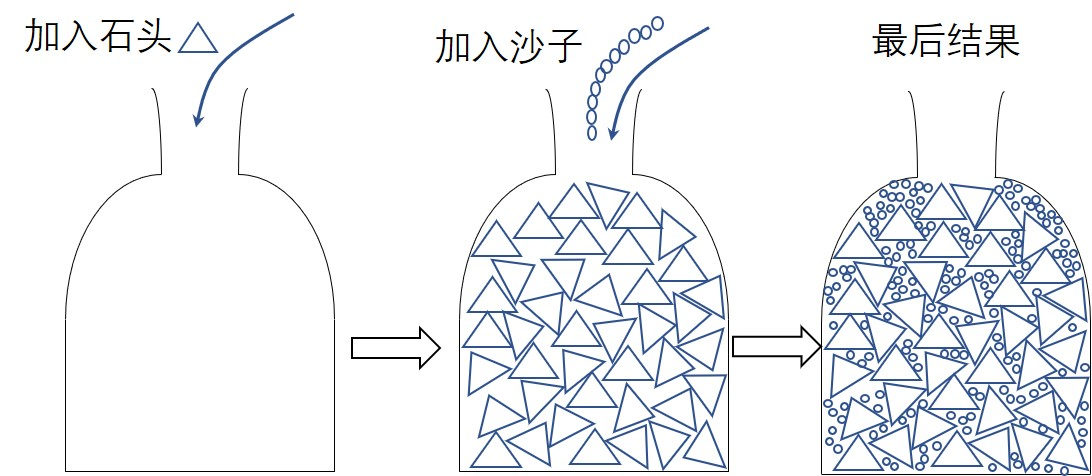
\includegraphics[width=.8\textwidth]{figures/shashi.jpg}
	 	\caption{沙石算法示意图}\label{shashi}
	 \end{figure}
	 
	 \paragraph{算法描述}
	 	\begin{itemize}
	 	\item [(1)] \textbf{装备均分}:将每个旅分解为连编制,即得到面积规划向量:
	 \begin{gather*}
	 	A^k=[a^k_{1},a^k_{2},\cdots,a^k_{n}]
	\end{gather*}
	 	其中$a^k_{i}$的初始值是第$k$旅中的全副武装人员所占面积,$k=1,2,\cdots,K$($K$为旅队编制总数),$n=n_{k}$($n_{k}$为$k$旅连编制总数)。根据题目中装备均匀分配的要求,重复检索向量$A^k$中的每一个元素,选择最小值$min \left \{ a_{i} \right \}$ (装备量最少的营)使得该连添加装备$X_{j}$,即令:
	 	\begin{gather*}
	   min \left \{ a_{i} \right \}=min \left \{ a_{i} \right \}+s_{xj}
	 	\end{gather*}
	 	重复检索直到该旅装备数$X=0$时,结束装备均分,得到装备均分后的部队$ \left \{A^k\right \}(k=1,2,\cdots,n_{k})$($n_{k}$为k旅连编制总数)。
	
		\item [(2)] \textbf{部队装载}:将装备均分后的部队$ \left \{A^k\right \}$中的元素混合后由大到小进行排序得到排序后的营编制总部对数列$ \left \{T_{n}\right \}$:
			\begin{gather*}
	T_{n}\geqslant 	T_{n+1}\\
	n\leq \sum_{1}^{K}n_{k}
		\end{gather*}
		将所有派出船舰装载面积进行排序得到船舰面积数列$ \left \{P_{n}\right \}$:
		依次检索总部对数列$ \left \{T_{n}\right \}$,并依次检索数列$ \left \{P_{n}\right \}$对应的船舰,将其装入剩余面积足够的船舰,即若$P_{n}\geqslant T_{n}$ 令:
		\begin{gather*}
		P_{n}=	P_{n}-	T_{n}
		\end{gather*}
		重复检索直到部队装载完成,即当部队检索次数$i=\sum_{1}^{K}n_{k}$时,算法结束。
		\item [(3)] \textbf{结果输出}:输出总共使用的船舰数量,即决策向量:
		\begin{gather*}
		D=[y_{1},y_{2},\cdots,y_{14},z_{1},z_{2},\cdots,z_{5}]
		\end{gather*}
	\end{itemize}
	%沙石算法的流程图如图~\ref{shashiluc}~
	 
\begin{figure}[H]
	\centering
	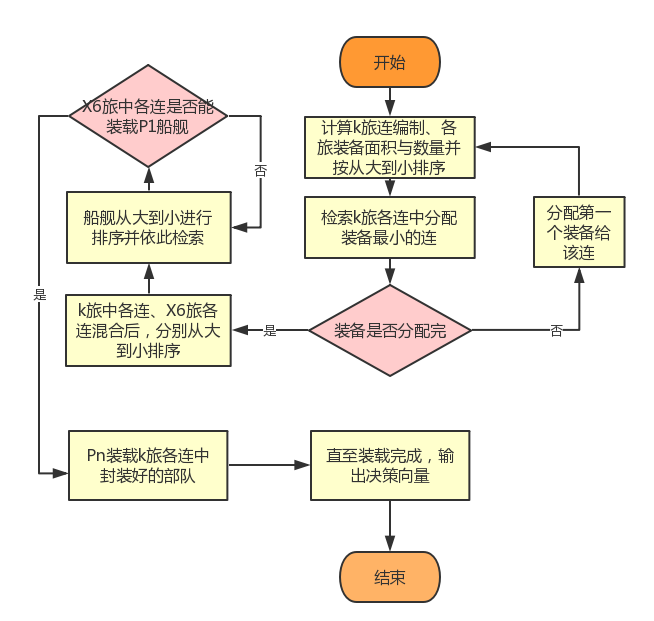
\includegraphics[width=.9\textwidth]{figures/shashisuanfa.png}
	\caption{沙石算法流程图}\label{shashiluc}
\end{figure}


\subsection{结果分析}
通过量化各型旅成建制单位的人数、装备面积和船舰的有效装载面积,结合相关条件和要求,再运用沙石算法进行计算,求解出各旅级单位装备人口面积装载方案如表~\ref{zhuangzai}~,其各连具体到每艘轮船数据见附件:

\begin{table}[H]
\centering		\caption{各型旅级单位装备人口面积装载方案}\label{zhuangzai}
\begin{tabular}{cccccc}
	\toprule[2pt]
	\multicolumn{1}{m{2cm}}{\centering 船舰类别}
	& \multicolumn{1}{m{2cm}}{\centering 第Ⅰ型旅}
	&\multicolumn{1}{m{2cm}}{\centering 第Ⅱ型旅}
	& \multicolumn{1}{m{3cm}}{\centering $ \cdots \cdots  $}
	& \multicolumn{1}{m{2cm}}{\centering 第Ⅺ型旅}
	& \multicolumn{1}{m{2cm}}{\centering 第Ⅻ型支队(旅)}
	\\
	\midrule[1pt]
	Y1综合登陆舰 &  $267.6285185$  &$0$ & $\cdots \cdots$&$5658.770914
	$ &$42.85714286$ \\ 
	Y2大型登陆舰	 &  $1586.951111$&$0$& $\cdots \cdots$ &$0$ &$0$\\ 
	Y3大型登陆舰	 &  $3178.042222 $ &$0$& $\cdots \cdots$ &$5864.014286
	$ &$0$\\ 
	Y4大型登陆舰	 &  $2114.508148 $ &$0$& $\cdots \cdots$ &$0
	$ &$0$\\ 
	$\cdots \cdots$	 &  $\cdots \cdots$  &$\cdots \cdots$ &$\cdots \cdots$ &$\cdots \cdots$ &$\cdots \cdots$\\ 
	Y12登陆艇	 &  $0$ &$0$ & $\cdots \cdots$ &$0$ &$728.5714286$\\ 
	Y13登陆艇	 &  $0$ &$0$ & $\cdots \cdots$ &$0$ &$0$\\ 
	Y14登陆艇		 &  $0$ &$0$ & $\cdots \cdots$ &$0$ &$0$\\ 
	2万吨级滚装船  &  $0 $ &$6549.897037$& $\cdots \cdots$ &$0$ &$0$ \\ 
	\bottomrule[2pt]	
\end{tabular}
\end{table}

	其各类舰船的使用数量与平均有效面积利用率$\frac{\sum P_{n}\cdot S_{k}}{\sum D*S_{n}*0.75}$如下表所示:
	\begin{table}[H]
		\centering		\caption{各类舰船的使用数量与平均有效面积利用率}\label{zhuansasgzai}
		\begin{tabular}{ccc}
			\toprule[2pt]
			\multicolumn{1}{m{3cm}}{\centering 船舰类别}
			& \multicolumn{1}{m{3cm}}{\centering 使用数目}
			&\multicolumn{1}{m{3cm}}{\centering 平均有效面积利用率}
			\\
			\midrule[1pt]
			Y1综合登陆舰 &  $5$  &$99.25$\% \\ 
			Y2大型登陆舰	 &  $3$&$94.04$\%\\ 
			Y3大型登陆舰	 &  $9 $ &$99.81$\%\\ 
			Y4大型登陆舰	 &  $4$ &$93.98$\%\\ 
			$\cdots \cdots$	 & 	$\cdots \cdots$&	$\cdots \cdots$\\ 
			Y12登陆艇	 &  $138$ &$70.38$\%\\ 
			2万吨级滚装船  &  $1 $ &$93.74$\% \\ 
			\bottomrule[2pt]	
		\end{tabular}
	\end{table}
由表~\ref{zhuansasgzai}~可知,由沙石算法设计的装备兵力装载方案,其有效面积利用率相当高,能大幅度减少船只数目填充更多武装兵力。
	
	
		
	\section{问题二模型的建立与求解}
	\subsection{问题的描述与分析}

	问题二要求针对具体运输任务,结合港口泊位,制定时间最短、船只数量最少的兵力装载方案。本组通过遗传算法,将问题一中的决策向量作为染色体,装载时间和船支数量作为适应度函数,建立装载方案优化模型。修改问题一中的沙石算法,作为验证算法判断每个个体是否可以存活,并随机生成$w$个能通过验证算法的初始个体。将某一代个体经过交叉、变异后的基因带入时间轴仿真模型,计算出装载所用时间作为适应度函数,将生成个体按照适应度函数大小进行第一次排序,再将装载所用时间大小相同的函数进行第二次排序,取出排序中前$w$个个体进行下一次进化,进化$g$代个体后可求得装载时间最短,同时使用海上运输工具最少的兵力装载方案。	                                                                                                   
	\subsection{模型的建立}
	    \subsubsection{优化函数与约束条件}
	基于问题一模型\textbf{决策向量}为:
	\begin{gather}
	D=[y_{1},y_{2},\cdots,y_{14},z_{1},z_{2},\cdots,z_{5}]
	\end{gather}
	\textbf{目标函数}为:
	\begin{gather}
	min Z=\sum _{1}^{19}D[k]
	\end{gather}
	增加\textbf{目标函数}:
		\begin{gather}
	min \left \{ \underset{k}{max}\sum t_{i} \right \}
	\end{gather}
	其中$\sum t_{i}(i=1,2\cdots,71)$,表示在共计$71$个泊口中第$i$个泊口的装载时间总和。	
		综上,建立得到问题二时间数量优化模型:
	\begin{gather}
	min Z=\sum _{1}^{19}D[k]\\
	min \left \{ \underset{k}{max}\sum t_{i} \right \}\\
	s.t.\left\{\begin{matrix}	 D\cdot S_{D}\geq \sum  S_{x} + \sum  S_{p}
	\\ y_{1}\cdot s_{y1}\geq \sum s_{x9}+ \sum  s_{p6}
	\\S_{D}=[S_{y}, S_{z}]
	\\ s_{xi}=l_{i}\times w_{i} \times \varepsilon _{i}
	\\S_{x}=[s_{x1},s_{x2},\cdots,s_{x14}]
	\\s_{pi}=p_{i}\times s
	\\S_{p}=[s_{p1},s_{p2},\cdots,s_{p12}]
	\\     s_{yi}=s_{i}\times \eta_{1}
	\\   S_{y}=[s_{y1},s_{y2},\cdots,s_{y14}]
	\\      s_{zj}=s_{j}\times \eta_{2}
	\\ S_{z}=[s_{z1},s_{z2},\cdots,s_{z5}]
	\end{matrix}\right. 
	\end{gather}
	其中$min \left \{ \underset{k}{max}\sum t_{i} \right \}$可利用\textbf{泊口仿真模型}计算,并通过\textbf{遗传算法}算得全局最优解。
	\subsubsection{泊口仿真模型}
	建立泊口仿真模型以计算每种方案的装载时间,首先输入决策向量:

		\begin{gather*}
	 D=[y_{1},y_{2},\cdots,y_{14},z_{1},z_{2},\cdots,z_{5}]
		\end{gather*}
	定义时间函数为$t_{0}$,初始化时间函数令$t_{0}=0$,并令$t_{0}$以$1$为步长逐渐增加。
	定义港口决策向量为:
		\begin{gather*}
		T=[t_{1},t_{2},\cdots,t_{71}]
		\end{gather*}
	$t_{k}(k=1,2,3,\cdots,71)$代表$71$个港口当前任务的结束时间。当$t_{k}=t_{0}$ 时,表示港口$k$处于空闲状态,此时立即更新任务结束时间$t_{k}$,即使得:
		\begin{gather*}
		t_{k}=t_{k}+t_{d}\\
		D[d]=D[d]-1
		\end{gather*}
	其中$t_{d}$是决策向量$D$中第$d$各元素对应船舰的装载时间,$D[d]$为决策向量$D$中的第$d$个元素。当
		\begin{gather*}
	\left\{\begin{matrix} \sum_{1}^{19}D[d]=0
	\\t_{0}\geqslant max t_{k} 	
	\end{matrix}\right.
		\end{gather*}

		即所有船支装载完成时,结束运算,输出当前的时间函数$t_{0}$,即:
			\begin{gather*}
		min \left \{ \underset{k}{max}\sum t_{i} \right \}=t_{0}
			\end{gather*}

	\subsubsection{遗传算法}
	 \paragraph{编码}
	 如图所示,每个个体由下面三个方块构成,其中最后一个进行遗传操作:
	 	\begin{figure}[H]
	 	\centering
	 	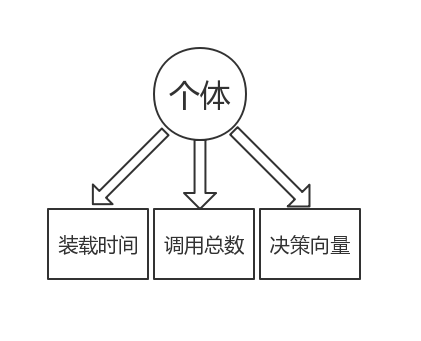
\includegraphics[width=.5\textwidth]{figures/yichuan.jpg}
	 	\caption{指标重要度占权图}\label{yichuan}
	 	 \end{figure}
	 根据题目要求,优先使用军用登陆舰,即决策向量$D=[y_{1},\cdots,y_{14},z_{1},\cdots,z_{5}]$中$y_{k}(k=1,2,\cdots,14)$为恒定值且等于其上限。故能简化决策向量为:
	\begin{gather*}
	D=[z_{1},z_{2}\cdots,z_{5}]
	\end{gather*}
	 \paragraph{交叉}
	 为保证变异率并保留优秀基因片段和本题采用的两种交叉方式:
	\begin{itemize}
	\item [(1)]: 单点交叉:对于两个父代个体$D=[z_{1},z_{2}\cdots,z_{5}]$和	$D'=[z_{1}',z_{2}'\cdots,z_{5}']$,随机选择第$k$个基因处为交叉点,将该基因后所有基因进行交换,得到子代基因
	\item [(2)]:中间值交叉:对于两个父代个体$D=[z_{1},z_{2}\cdots,z_{5}]$和	$D'=[z_{1}',z_{2}'\cdots,z_{5}']$,随机选取$z_{k}''\in [z_{k},z_{k}']$得到子代基因。
    \end{itemize}
    再选取交叉个体时采用混合分组的方法,将父代均匀混合后选取所有编号为奇数的个体,与其相邻对应编号为偶数的个体,通过两种交叉方式产生处两种类型的子代。
     \paragraph{变异}
     为保证种群多样性,以$0.1$的变异率,对选择的个体执行变异操作。随机选择变异个体中的基因$z_{k}$,使其值以各$50\%$的概率加一或减一。
     \paragraph{筛重}
     由于该模型基因维度较低,有大概率出现基因重复的个体,其对种群多样性有不利影响,并易使算法早熟。故在每次交叉变异生成新个体时删除重复基因,以提高算法的全局搜素能力。
     \paragraph{选择}
     由于本题约束条件较多,且有两个包含两个适应度函数,故采用两种选择方式:
     \begin{itemize}
     \item [(1)] \textbf{约束淘汰:}对于生成的个体基因$D=[z_{1},z_{2}\cdots,z_{5}]$带入第一问的沙石算法中,计算部队是否可以完全装入船支中。若不能则删除个体,若能则保留个体。
     \item [(2)]\textbf{精英选择:}由于模型假设战场上使用较少的时间优先级高于使用更少船支,将每一代中的生成个体与上一代混合,的个体按照其\textbf{装载时间}由大到小进行\textbf{第一次排序},再将装载时间相同的个体进行依照\textbf{调用总数}进行\textbf{第二次排序}。保留前列的$w$个个体,$w$为设定的种群容纳量。
     \end{itemize}
     重复上述进化过程,当进化代数足够多时,求解得到全局最优解。

     \subsection{模型的求解}
   	 \paragraph{算法的实现}
   	 	\begin{itemize}
   	 	\item [(1)]: 将染色体中的单个基因取出,带入问题一沙石算法中。计算只使用的某种民用船时,需要的该民用船的数量,作为单个基因的取值范围。在使用卡特蒙洛法随机生成初始个体,当生成$50$个能通过沙石算法检验的初始个体时,停止生成。
   	 	\item [(2)]:将输入体进行、交叉、变异、筛重和约束淘汰后,得到子代生成个体。将子代个体与附带个体混合,带入泊口仿真模型求出每个个体的装载时间作为适应度函数。根据装载时间对每个个体进行第一次排序,并将装载时间相同的个体进行第二次排序,取序列中的前$50$个个体作为下一代输入个体。
   	 	\item [(3)]:重复上述步骤(2),当进化次数达到$100$次时结束进化,选取当前最优个体作为输出个体,将输出个体基因与军用登陆舰合并即可得到完整的船支调遣方案。
   	 	 \end{itemize}
     \paragraph{算法流程图}
     
     
     \section{问题三模型的建立与求解}
   	\subsection{问题的描述与分析}
   	问题三要求,当装载行动开始24小时后,A港和D港有部分泊位被毁,给出调整方案和装载建议。
   	本组基于问题二中模型求解的结果,作出合理假设,假设泊位被毁不损失船只和兵力,由于问题二中的装载时间最优解小于$24$小时,故将码头被摧毁时间改为第$18$小时。本组延用问题二中的遗传算法,当时间轴进行到$18$小时,剔除已经完成装载任务的船舰和A港、D港中部分被毁的码头泊位,修改问题二中的港口仿真模型。通过遗传算法求解出对剩余船舰、码头泊位的装载方案,给出装载建议。
   	
   	
  \subsection{模型的建立}
    \subsubsection{模型调整}
    \textbf{优化函数与约束条件}延用问题二模型:
     	\begin{gather}
     min Z=\sum _{1}^{19}D[k]\\
     min \left \{ \underset{k}{max}\sum t_{i} \right \}\\
     s.t.\left\{\begin{matrix}	 D\cdot S_{D}\geq \sum  S_{x} + \sum  S_{p}
     \\ y_{1}\cdot s_{y1}\geq \sum s_{x9}+ \sum  s_{p6}
     \\S_{D}=[S_{y}, S_{z}]
     \\ s_{xi}=l_{i}\times w_{i} \times \varepsilon _{i}
     \\S_{x}=[s_{x1},s_{x2},\cdots,s_{x14}]
     \\s_{pi}=p_{i}\times s
     \\S_{p}=[s_{p1},s_{p2},\cdots,s_{p12}]
     \\     s_{yi}=s_{i}\times \eta_{1}
     \\   S_{y}=[s_{y1},s_{y2},\cdots,s_{y14}]
     \\      s_{zj}=s_{j}\times \eta_{2}
     \\ S_{z}=[s_{z1},s_{z2},\cdots,s_{z5}]
     \end{matrix}\right. 
     \end{gather}
     调整 \textbf{泊口仿真模型},延用港口决策向量:
     \begin{gather*}
     T=[t_{1},t_{2},\cdots,t_{71}]
     \end{gather*}
     当时间轴函数$t_{0}=18$时,停止被毁泊口正在进行的任务,即使
     \begin{gather}
     t_{k}=18(k=1,2,11,37,46,47)
     \end{gather}
     且之后检索港口决策向量时,剔除$ t_{k}(k=1,2,11,37,46,47)$。并将修改后泊口仿真模型算得的装载时间,带入遗传算法的适应度函数值,重新运行遗传算法。即可求得装载中途港口被摧毁后的最优船舰调整方案。
       \subsection{模型的求解}
     \paragraph{算法的实现}
     \paragraph{算法流程图}

	

	
	\subsection{结果分析}
     



	\section{模型的评价}
	\subsection{模型的优点}
		\begin{itemize}                                             
		\item [(1)] 将多目标优化转换成背包优化问题,自主设计沙石算法,使得船舰的面积利用率高,对船只数量的需求量少。
		\item [(2)] 
	
	\end{itemize}
	\subsection{模型的缺点}
	\begin{itemize}                                             
		\item [(1)] 
		\item [(2)] 
	\end{itemize}
	\subsection{模型改进}
	
    
	\newpage	%换页符
	%%参考文献
	%\begin{thebibliography}{9}%宽度9
	% \setlength{\itemsep}{-2mm}
	\nocite{*}		%排版未引用的参考文献
%\bibliography{wenxian.bib}
%	%参考文献添加到wenxian.bib里,再引用
%	
\begin{thebibliography}{9}%宽度9
	\bibitem{bib:one} Tan Jing Wei,Chang Siow-Wee,Binti Abdul Kareem Sameem,Yap Hwa Jen,Yong Kien-Thai. Deep Learning for Plant Species Classification using Leaf Vein Morphometric.[J]. IEEE/ACM transactions on computational biology and bioinformatics,2018.
	\bibitem{bib:two}Liu Jing,Sun Wanning,Su Yuting,Jing Peiguang,Yang Xiaokang. BE-CALF: Bit-Depth Enhancement by Concatenating All Level Features of DNN.[J]. IEEE transactions on image processing : a publication of the IEEE Signal Processing Society,2019,28(10).
	\bibitem{bib:three}Matheus B. Vicari,Mathias Disney,Phil Wilkes,Andrew Burt,Kim Calders,William Woodgate. Leaf and wood classification framework for terrestrial LiDAR point clouds[J]. Methods in Ecology and Evolution,2019,10(5).
	\bibitem{bib:}田德红,何建敏.基于变异粒子群优化与深度神经网络的航空弹药消耗预测模型[J].南京理工大学学报,2018,42(06).
	\bibitem{bib:}原继东,王志海,韩萌,游洋. 基于逻辑shapelets转换的时间序列分类算法[J]. 计算机学报,2015,38(07):1448-1459.
	\bibitem{bib:}杨志辉,胡红萍,白艳萍. 基于主成分分析和PSO-SVM的树叶分类方法研究[J]. 数学的实践与认识,2016,46(18):170-175.
	\bibitem{bib:}侯铜,姚立红,阚江明.基于叶片外形特征的植物识别研究[J].湖南农业科学,2009(04):123-125+129.
	\bibitem{bib:}Febri Liantoni,Rifki Indra Perwira,Syahri Muharom,Riza Agung Firmansyah,Akhmad Fahruzi. Leaf classification with improved image feature based on the seven moment invariant[J]. Journal of Physics: Conference Series,2019,1175(1).
\end{thebibliography}

	\newpage
	%附录
	\appendix %%附录

\section{代码}
\subsection{图片名称读取--matlab源代码}
\begin{lstlisting}[language=matlab]

\end{lstlisting}

\end{document}